%%%%%%%%%%%%
%
% $Autor: Chantal Crety $
% $Datum: 11.07.2025 $
% $Pfad: DemonstratorSchrittmotor\MontageAnleitung\Montage.tex
% $Beschreibung: Hauptteil der MontageAnleitung
%
%%%%%%%%%%%%



\chapter{Gehäuse}

\section{Fertigung}

Die Gehäuseteile werden mithilfe einer CAD-Software konstruiert und als STL-Dateien exportiert. Anschließend erfolgt die Aufbereitung der Daten mit einer Slicer-Software, um sie an den jeweiligen 3D-Drucker anzupassen. Nach der Slicer-Bearbeitung können die G-Codes erzeugt und an den 3D-Drucker übertragen werden, woraufhin der Druckprozess gestartet werden kann.Die STL-Dateien sind unter dem Pfad: \emph{DemonstratorSchrittmotor \textbackslash MontageAnleitung \textbackslash 3D-Print \textbackslash STL} zu finden. Wenn Sie den Original Prusa i3 MK3S+ Drucker verwenden, finden Sie die fertigen G-Codes unter dem Pfad: \emph{DemonstratorSchrittmotor \textbackslash MontageAnleitung \textbackslash 3D-Print \textbackslash GCode}. Falls Veränderungen an den original CAD Dateien erfolgen sollen, finden Sie diese für das Programm Fusion unter dem Pfad: \emph{DemonstratorSchrittmotor \textbackslash MontageAnleitung \textbackslash 3D-Print \textbackslash CAD}.

\section{3D-Druckteile}
Die Konstruktion des Gehäuses besteht aus zwei Aufsteckplatten und zwei Gehäusehälften. Die Aufsteckplatten sind für den Bereich zwischen den Profilen vorgesehen und bilden zusammen mit der vorhandenen Steuerplatine samt Montageplatte eine Rückwand. Diese schützt die Elektronik vor Schmutz und bietet gleichzeitig eine Fläche zur Befestigung elektronischer Komponenten.
Die Gehäusehälften bieten Platz für die Kabelführung, schützen das Innenleben und halten alle wichtigen Elemente sicher in Position.

\begin{minipage}{0.48\textwidth}
	\begin{figure}[H]
		\centering
		\begin{tikzpicture}[scale=1.4]
			\tikzstyle{every node}=[font=\LARGE]
			\draw [line width=1pt, short] (5.25,10.5) -- (5.5,10.5);
			\draw [line width=1pt, short] (5.5,7.5) -- (5.75,7.5);
			\draw [line width=1pt, short] (5.5,10.5) -- (5.75,7.5);
			\draw [line width=1pt, short] (5.25,10) -- (5,10);
			\draw [line width=1pt, short] (5.25,10.5) -- (5,10.5);
			\draw [line width=1pt, short] (5,10) -- (5,10.5);
			\draw [line width=1pt, short] (5,10.5) -- (5.5,10.75);
			\draw [line width=1pt, short] (5.5,10.75) -- (5.75,10.75);
			\draw [line width=1pt, short] (7.25,11.75) -- (7.75,12);
			\draw [line width=1pt, short] (5.25,7.5) -- (5.5,7.5);
			\draw [line width=1pt, short] (5.25,7.75) -- (5.25,7.5);
			\draw [line width=1pt, short] (5.25,7.75) -- (5.5,7.75);
			\draw [line width=1pt, short] (5.25,7.75) -- (5.5,8);
			\draw [line width=1pt, short] (5.5,7.75) -- (5.25,10);
			\draw [line width=1pt, short] (5.75,7.5) -- (8.5,9.25);
			\draw [line width=1pt, short] (8.5,9.25) -- (8.25,12);
			\draw [line width=1pt, short] (5.5,10.5) -- (8.25,12);
			\draw [line width=1pt, short] (7.75,12) -- (8.25,12);
			\draw [line width=1pt, short] (5.75,10.75) -- (7.5,11.75);
			\draw [line width=1pt, short] (7.25,11.75) -- (7.5,11.75);
		\end{tikzpicture}
		\caption{Platte groß}
		\label{fig:platte_gross}
	\end{figure}
\end{minipage}
\hfill
\begin{minipage}{0.48\textwidth}
	\begin{figure}[H]
		\centering
		\begin{tikzpicture}[scale=0.6]
			\tikzstyle{every node}=[font=\LARGE]
			\draw [line width=1pt, short] (10,5.25) -- (10.25,-2);
			\draw [line width=1pt, short] (10,5.25) -- (15,7.75);
			\draw [line width=1pt, short] (10.25,-2) -- (15.25,1);
			\draw [line width=1pt, short] (15.25,1) -- (15,7.75);
			\draw [line width=1pt, short] (10,5.25) -- (9.25,5.5);
			\draw [line width=1pt, short] (15,7.75) -- (14.25,8);
			\draw [line width=1pt, short] (10.25,-2) -- (9.5,-1.5);
			\draw [line width=1pt, short] (9.5,-0.75) -- (9.5,-1.5);
			\draw [line width=1pt, short] (9.5,-0.75) -- (9.75,-1);
			\draw [line width=1pt, short] (9.5,4.75) -- (9.75,-1);
			\draw [line width=1pt, short] (9.25,5.5) -- (9.25,4.5);
			\draw [line width=1pt, short] (9.25,4.5) -- (9.5,4.75);
			\draw [line width=1pt, short] (9.25,5.5) -- (10.25,6);
			\draw [line width=1pt, short] (14.25,8) -- (13.25,7.5);
			\draw [line width=1pt, short] (13.25,7.5) -- (13.5,7.5);
			\draw [line width=1pt, short] (13.5,7.5) -- (10.5,6);
			\draw [line width=1pt, short] (10.25,6) -- (10.5,6);
			\draw [line width=1pt, short] (9.5,-0.75) -- (9.75,-0.5);
			\draw [line width=1pt] (12.25,3.75) ellipse (0.25cm and 0.25cm);
			\node [font=\LARGE] at (12.75,3.75) {};
			\draw [line width=1pt] (12.25,2) ellipse (0.25cm and 0.25cm);
			\draw [line width=1pt, short] (12.25,4) .. controls (12.5,3.75) and (12.25,3.75) .. (12.25,3.5);
			\draw [line width=1pt, short] (12.25,2.25) .. controls (12.5,2) and (12.25,2) .. (12.25,1.75);
		\end{tikzpicture}
		\caption{Platte klein}
		\label{fig:platte_klein}
	\end{figure}
\end{minipage}

	\vspace{0.5cm}

\begin{figure}[H]
	\centering
\begin{tikzpicture}[scale=0.6]
	\tikzstyle{every node}=[font=\LARGE]
	\draw [line width=1pt] (10.5,2.75) -- (20.25,5);
	\draw [line width=1pt] (5.75,10) -- (7.5,10.25);
	\draw [line width=1pt] (5.75,10) -- (9,8);
	\draw [line width=1pt] (9,8) -- (9,6.25);
	\draw [line width=1pt] (5.75,10) -- (5.75,8.25);
	\draw [line width=1pt] (10,8) -- (6.75,9.75);
	\draw [line width=1pt] (6.75,9.75) -- (8,10);
	\draw [line width=1pt] (7.5,10.25) -- (8,10);
	\draw [line width=1pt] (7.75,4.75) -- (7.75,7);
	\draw [line width=1pt] (8,9.25) -- (8,9.75);
	\draw [line width=1pt] (7.75,4.75) -- (10.5,2.75);
	\draw [line width=1pt] (10.5,2.75) -- (10.5,9);
	\draw [line width=1pt] (10.5,9) -- (20.25,10.5);
	\draw [line width=1pt] (20.25,5) -- (20.25,10.5);
	\draw [line width=1pt] (7.75,10.5) -- (7.75,9.25);
	\draw [line width=1pt] (6.5,7.75) -- (7,8.25);
	\draw [line width=1pt] (7,8.25) -- (8,7.75);
	\draw [line width=1pt] (8,7.75) -- (8,7);
	\draw [line width=1pt] (6.5,7.75) -- (5.75,8.25);
	\draw [line width=1pt] (8,7) -- (9,6.25);
	\draw [line width=1pt] (6.5,7.75) -- (7.75,7.75);
	\draw [line width=1pt] (7.75,8) -- (7.75,7);
	\draw [line width=1pt] (10.5,9) -- (7.75,10.5);
	\draw [line width=1pt] (7.75,10.5) -- (17.25,11.75);
	\draw [line width=1pt] (20.25,10.5) -- (17.25,11.75);
	\draw [line width=1pt] (9,6.25) -- (10,6);
	\draw [line width=1pt] (9,8) -- (10,7.75);
    \draw [line width=1pt] (10,7.75) -- (10,6);
    \draw [line width=1pt] (10,8) -- (10,7.75);
    \end{tikzpicture}
	
	\caption{Körper links}
	\label{tikz:Kl}
\end{figure}

\begin{figure}[H]
	\vspace{0.5cm}
	\centering
	\begin{tikzpicture}[scale=1.6]
		\tikzstyle{every node}=[font=\LARGE]
	    \draw[line width=1pt] (5,11) rectangle (10,8.75);
		\draw [line width=1pt] (10,11) -- (10.5,11.5);
		\draw [line width=1pt] (10,8.75) -- (10.5,9.25);
		\draw [line width=1pt] (10.25,10.75) -- (11,11.5);
		\draw [line width=1pt] (11,11.5) -- (10.5,11.5);
		\draw [line width=1pt] (10.25,11.5) -- (10.75,11.75);
		\draw [line width=1pt] (10.75,11.75) -- (11.5,11.75);
		\draw [line width=1pt] (11.5,11.75) -- (10.75,10.75);
		\draw [line width=1pt] (10.75,10.75) -- (10.25,10.5);
		\draw [line width=1pt] (10.25,10.5) -- (10.25,9.75);
		\draw [line width=1pt] (10.25,9.75) -- (10.75,10);
		\draw [line width=1pt] (10.75,10.75) -- (10.75,10);
		\draw [line width=1pt] (10.75,10) -- (11.5,11);
		\draw [line width=1pt] (11.5,11.75) -- (11.5,11);
		\draw [line width=1pt] (10.5,11.5) -- (10.5,11);
		\draw [line width=1pt] (5,11) -- (6,11.5);
		\draw [line width=1pt] (10.5,11.5) -- (6,11.5);
		\draw [line width=1pt] (10.5,9.75) -- (10.5,9.25);
		\draw [line width=1pt] (9,11) -- (9.25,11.25);
		\draw [line width=1pt] (9.25,11.25) -- (9.75,11.25);
		\draw [line width=1pt] (9.25,11.25) -- (9.5,11.25);
		\draw [line width=1pt] (9.75,11.25) -- (9.5,11);
		\draw [line width=1pt] (9.25,11.25) -- (9.75,11.25);
		\draw[line width=1pt] (8,10) circle (0.25cm);
		\draw[line width=1pt] (9.25,10) circle (0.12cm);
		\draw[line width=1pt] (9.25,9.5) circle (0.12cm);
		\draw[line width=1pt] (5.75,10.75) rectangle (7.25,10);
		\draw [line width=1pt] (9.25,11.25) -- (9.5,11.25);
		\draw [line width=1pt] (9.5,11.25) -- (9.75,11.25);
		\draw [line width=1pt] (9.25,11) -- (9.5,11);
		\draw [line width=1pt] (9.25,11) -- (9.5,11);
	\end{tikzpicture}
	\caption{Körper rechts}
	\label{tikz:KR}
\end{figure}



\raggedright

\chapter{Vorbereitung der Elektronik}

\section{Programmierung des Arduino Nano 33 BLE Sense Rev.2}
Die Programmierung des Schrittmotors erfolgt mit dem Arduino Nano 33 BLE Sense Rev.2, im weiteren Verlauf dieses Dokuments als Arduino bezeichnet. Dazu wird die Entwicklungsumgebung Arduino IDE in Verbindung mit einem USB-Kabel und dem Arduino verwendet.\\

Eine Einführung in die Programmstruktur sowie die Einrichtung der Arduino-Umgebung finden Sie im Verzeichnis:
\emph{DemonstratorSchrittmotor \textbackslash Nano33BLESense \textbackslash Contents \textbackslash General}.

Nach Durcharbeitung der Einführung kann die eigentliche Programmierung im angegebenen \emph{DemonstratorSchrittmotor \textbackslash Nano33BLESense \textbackslash Code \textbackslash Arduino \textbackslash Demonstrator Schrittmotor} gefunden, in die Arduino IDE importiert und anschließend auf den Arduino hochgeladen werden. 


\section{Anbringung der Lochscheibe des Geschwindigkeitssensors LM393}

Zur Messung der Geschwindigkeit wird die Lochscheibe des Sensors an der Stirnfläche der freiliegenden Spindel befestigt. Dies geschieht über die genaue Ausrichtung des Zylinderschraubenkopfes und einer Lötverbindung zwischen dieser und der Spindel. Eine mittige und horizontale Ausrichtung ist hierbei gefordert. Zur Kontrolle der Befestigung kann die Spindel händisch gedreht werden. Bei einem unrunden Drehlauf, kann das Lötmaterial erhitzt und eine erneute Ausrichtung durchgeführt werden. Treten nach mehreren Korrekturversuchen Haftungsprobleme auf, wird eine gründliche Entfettung und Aufrauung der Kontaktflächen empfohlen.


\begin{figure}[H]
	\vspace{0.5cm}
	\centering
	\begin{tikzpicture}[
		scale=0.2,
		every node/.style={font=\fontsize{8pt}{10pt}\selectfont\bfseries}
		]
		\draw [ line width=1pt ] (14.5,10) rectangle (16.75,-16.75);
		\draw [ line width=1pt , dashed] (14.5,2) rectangle  (16.75,0.75);
		\draw [ line width=1pt ] (14.5,2) rectangle (4,0.75);
		\draw [ line width=1pt ] (16.75,2) rectangle (17.5,0.75);
		\draw [ line width=1pt ] (17.5,1.75) rectangle (19.5,1);
		\draw [line width=1pt] (9,0.75) -- (10,-12);
		\draw [line width=1pt] (16.75,-8.25) -- (17,-11.75);
		\draw [line width=1pt] (18.5,1) -- (20.25,-11.75);
		\draw [line width=1pt] (16.75,0.75) -- (18.5,-11.75);
		
		% Knoten mit angepasster Schrift
		\node at (10,-12.5) {1};
		\node at (17,-12.5) {2};
		\node at (18.5,-12.5) {3};
		\node at (20.25,-12.5) {4};
		
	\end{tikzpicture}
	
	1 - Spindel; 2 - Frästischseite rechts; 3 - Lötzinn; 4 - Zylinderkopfschraube M5; 
	
	\caption{Achsausrichtung der Lochscheibe}
	\label{tikz:LScheibe}
\end{figure}

\raggedright


\begin{figure}[H]
	\vspace{1.5cm}
	\centering
	\tikzset{short/.style={}}
	\begin{tikzpicture}[scale=0.2, xscale=-1,
		every node/.style={font=\fontsize{800pt}{1000pt}\selectfont\bfseries}] 
		\tikzstyle
		\draw [ line width=1pt ] (31.5,-0.75) ellipse (4.5cm and 9cm);
		\draw [ line width=1pt , rotate around={90:(31.5,-0.75)}] (31.5,-0.75) ellipse (1.5cm and 1cm);
		\draw [ line width=1pt , rotate around={90:(39.5,-0.5)}] (39.5,-0.5) ellipse (1.5cm and 1cm);
		\draw [ fill={rgb,255:red,253; green,253; blue,253} , line width=1pt ] (51.25,-0.75) ellipse (2.25cm and 3.25cm);
		\draw [ line width=1pt , rotate around={90:(51.25,-0.75)}] (51.25,-0.75) ellipse (1.5cm and 1cm);
		\draw [line width=1pt, short] (48.5,2.75) -- (51.25,2.5);
		\draw [line width=1pt, short] (48,-3.75) -- (51,-4);
		\draw [line width=1pt, short] (43.25,1) -- (46.5,1);
		\draw [line width=1pt, short] (43,-2) -- (46.5,-2.25);
		\draw [line width=1pt, short] (43,-2) .. controls (42.25,-1.25) and (42.25,0.5) .. (43.25,1);
		\draw [line width=1pt, short] (29.75,8.5) -- (31.75,8.25);
		\draw [line width=1pt, short] (29.75,-9.5) -- (31.25,-9.75);
		\draw [line width=1pt, short] (48.5,2.75) .. controls (46.25,2.75) and (45,-2) .. (48,-3.75);
		\draw [line width=1pt, short] (29.75,8.5) .. controls (23.75,6) and (25,-8.25) .. (29.75,-9.5);
		\draw [ line width=1pt ] (31.5,-0.75) ellipse (2cm and 3.75cm);
		\draw [ line width=1pt ] (31.5,-0.75) ellipse (4cm and 8.5cm);
		\draw [line width=1pt, short] (31.5,7.75) -- (31.5,3);
		\draw [line width=1pt, short] (31.25,7.75) -- (31.25,3);
		\draw [line width=1pt, short] (31.5,-4.5) -- (31.5,-9.25);
		\node [font=\LARGE] at (32,5) {};
		\node [font=\LARGE] at (32.25,4.5) {};
		\draw [line width=1pt, short] (31.25,-4.5) -- (31.25,-9.25);
		\draw [line width=1pt, short] (31,0.5) .. controls (32,-0.25) and (31.5,-1.5) .. (31,-2);
		\draw [line width=1pt, short] (33.5,6.5) -- (32.5,2.5);
		\draw [line width=1pt, short] (33.75,6.25) -- (32.75,2.25);
		\node [font=\LARGE] at (33.5,4) {};
		\draw [line width=1pt, short] (30.5,-4) -- (29.5,-8);
		\draw [line width=1pt, short] (30.75,-4.25) -- (29.75,-8.25);
		\draw [line width=1pt, short] (32.25,-4.25) -- (33.75,-7.75);
		\draw [line width=1pt, short] (29.25,6.25) -- (30.5,2.5);
		\draw [line width=1pt, short] (32.5,-4) -- (34,-7.5);
		\draw [line width=1pt, short] (29,6) -- (30.25,2.25);
		\draw [line width=1pt, short] (28,3) -- (29.75,1.25);
		\draw [line width=1pt, short] (27.75,2.5) -- (29.75,0.75);
		\draw [line width=1pt, short] (33.25,-3) -- (35.25,-4.25);
		\draw [line width=1pt, short] (33.25,-2.5) -- (35.25,-3.75);
		\draw [line width=1pt, short] (33.25,1.5) -- (35,3);
		\draw [line width=1pt, short] (33.25,1) -- (35.25,2.75);
		\draw [line width=1pt, short] (33.5,-0.25) -- (35.5,0);
		\draw [line width=1pt, short] (33.5,-0.75) -- (35.5,-0.5);
		\draw [line width=1pt, short] (27.5,-1) .. controls (28.25,-0.75) and (28.5,-0.75) .. (29.5,-0.75);
		\draw [line width=1pt, short] (27.5,-1.5) .. controls (28.25,-1.25) and (28.5,-1.25) .. (29.5,-1.25);
		\draw [line width=1pt, short] (28,-5) -- (29.75,-2.75);
		\draw [line width=1pt, short] (28.25,-5.5) -- (30,-3);
		\draw [ line width=1pt , rotate around={90:(23.5,-0.75)}] (23.5,-0.75) ellipse (1.5cm and 1cm);
		\draw [ line width=1pt ] (39.5,-0.5) ellipse (2.5cm and 4.5cm);
		\draw [line width=1pt, short] (38.5,4) .. controls (35.25,2.75) and (36.25,-4.75) .. (38.75,-5);
		\draw [line width=1pt, short] (39.5,4) -- (38.5,4);
		\draw [line width=1pt, short] (39.5,-5) -- (38.75,-5);
		\draw [line width=1pt, short] (39.5,1) .. controls (40.5,0.25) and (40.5,-1.25) .. (39.5,-2);
		\draw [line width=1pt, short] (23,0.5) .. controls (23.75,0.25) and (23.75,-1.25) .. (23,-2);
		\draw [line width=1pt, short] (22.25,2) -- (21.25,0);
		\draw [line width=1pt, short] (21.25,0) -- (21.5,-2.25);
		\draw [line width=1pt, short] (22.25,2) -- (24.5,2);
		\draw [line width=1pt, short] (24.5,2) -- (25.5,0.5);
		\draw [line width=1pt, short] (25.5,0.5) -- (25.5,-2);
		\draw [line width=1pt, short] (25.5,-2) -- (24.5,-3.5);
		\draw [line width=1pt, short] (21.5,-2.25) -- (22.5,-3.5);
		\draw [line width=1pt, short] (22.5,-3.5) -- (24.5,-3.5);
		\draw [line width=1pt, short] (24.5,2) -- (22.25,2.25);
		\draw [line width=1pt, short] (24.5,-3.5) -- (21.25,-3.75);
		\draw [line width=1pt, short] (21.25,0) -- (19.5,0);
		\draw [line width=1pt, short] (21.5,-2.25) -- (19.75,-2.25);
		\draw [line width=1pt, short] (19.5,0) -- (19.75,-2.25);
		\draw [line width=1pt, short] (19.75,-2.25) -- (21.25,-3.75);
		\draw [line width=1pt, short] (22.25,2) -- (20.75,2);
		\draw [line width=1pt, short] (19.5,0) -- (20.75,2);
		\draw [line width=1pt, short] (21.25,-3.75) -- (22.5,-3.5);
		\draw [line width=1pt, short] (20.75,2) -- (22.25,2.25);
		\draw [line width=1pt, short] (30.5,-9.5) -- (29,-14.25);
		\draw [line width=1pt, short] (39.25,-5) -- (36.5,-13.75);
		\draw [line width=1pt, short] (49,-3.75) -- (45,-14);
		\draw [line width=1pt, short] (22.5,-3.75) -- (19.5,-14);
		\node [xscale=-1, transform shape] at (28.75,-15.25) {3};
		\node [xscale=-1, transform shape] at (36,-15) {2};
		\node [xscale=-1, transform shape] at (44.75,-15) {1};
		\node [xscale=-1, transform shape] at (19.25,-15) {4};
	\end{tikzpicture}
	\vspace{1cm}
	
	1 - Zylinderkopfschraube M5; 2 - Unterlegscheibe M5; 3 - Lochscheibe; 4 - Mutter M5; 
	
	\caption{Reihenfolge der Lochscheiben Anbringung}
	\label{tikz:LScheibe}
\end{figure}
\raggedright

Zur Montage der Lochscheibe wird diese zusammen mit einer Unterlegscheibe und Mutter auf der Schraube handfest angezogen. Dies ist in der Abbildung 4.2 dargestellt.

\section{Veränderung der Display Steuerung}
Das Display kann über vier verschiedene Schnittstellen gesteuert werden: I2C, SPI, 8-Bit Parallel 6800 und 8-Bit Parallel 8080. Für unser Projekt wird die I2C-Schnittstelle benötigt.[...]

Um diese auszuwählen, müssen die Widerstände auf der Rückseite des Displays mithilfe eines Lötkolbens umgelötet werden. Dabei ist besonders darauf zu achten, mit Vorsicht zu arbeiten, da die Widerstände sehr klein und leicht sind.[...]

Verlöten Sie die Widerstände auf BS1 - 1 und BS2 - 0.



\begin{table}[h]
	\centering
	\begin{tabular}{lcccc}
		\hline
		& I2C & SPI & 8 Bit parallel 6800 & 8 Bit parallel 8080 \\
		\hline
		BS1 & 1 & 0 & 0 & 1 \\
		BS2 & 0 & 0 & 1 & 1 \\
		\hline
	\end{tabular}
	\caption{Display Schnittstellen}
	\label{tab:bs_schnittstellen}
\end{table}

	\vspace{-1.5cm}

\begin{figure}[H]
	\begin{center}
		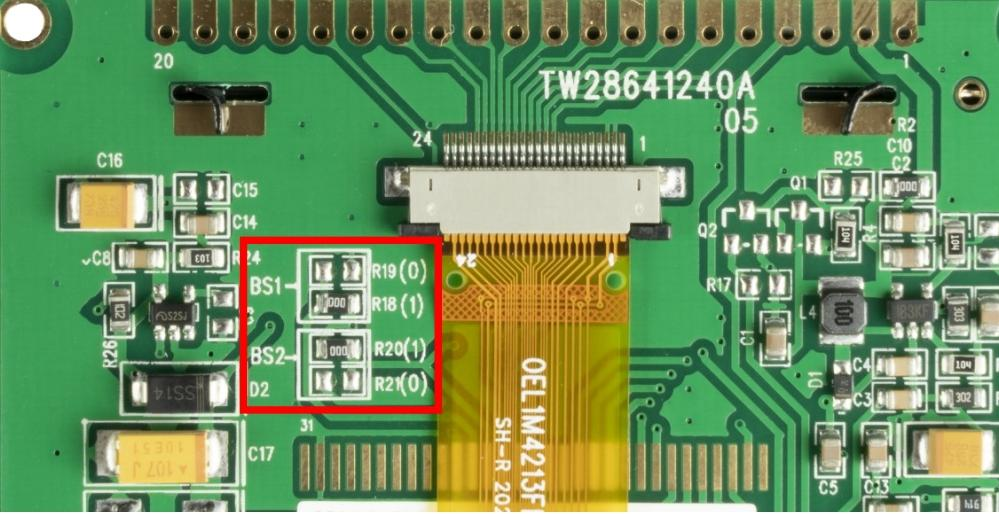
\includegraphics[width=0.7\textwidth]{Images/DisplayRückseite.jpg}
		\caption{Schaltplan} \label{DisplayRückseite}
	\end{center}
\end{figure}

\section{Vorbereitung der elektrischen Leitungen}

Die elektrischen Leitungen werden im Vorfeld vorbereitet, um einen reibungslosen Montageprozess zu gewährleisten. Die benötigten Kabel sowie deren Anschlussarten, Längen und Bezeichnungen sind in Tabelle \ref{Leittab} aufgeführt. Bitte bereiten Sie die Kabel entsprechend für die folgenden Arbeitsschritte vor, indem Sie alle Leitungen mit der ersten Anschlusskomponente verbinden. Dies erfolgt, im Fall von Female-/Male-Anschlüssen über den Steckmechanismus, oder durch Schnüren und Anlöten der Leitungen an Schaltern bei abisolierten Verbindungen. Zur besseren Übersicht wird empfohlen, Leitungen mit gleicher Funktion in derselben Farbe zu verwenden.

\textbf{Sicherheitshinweise zum Umgang mit dem Lötkolben}

Beim Arbeiten mit dem Lötkolben ist besondere Vorsicht geboten, da hohe Temperaturen zu Verletzungen oder Schäden an elektronischen Komponenten führen können. Beachten Sie daher folgende Sicherheitshinweise:

\begin{itemize}
	\item Verwenden Sie den Lötkolben ausschließlich auf einer hitzebeständigen Unterlage und in einem gut belüfteten, windstillen Arbeitsbereich.
	\item Halten Sie ausreichend Abstand zu brennbaren Materialien.
	\item Schalten Sie den Lötkolben nach Gebrauch sofort aus und lassen Sie ihn vollständig abkühlen, bevor Sie ihn weglegen oder verstauen.
	\item Achten Sie beim Entlöten darauf, benachbarte Bauteile nicht zu überhitzen oder die Leiterbahnen zu beschädigen.
	\item Lassen Sie den Lötkolben niemals unbeaufsichtigt in eingeschaltetem Zustand.
\end{itemize}

Befolgen Sie diese Hinweise sorgfältig, um eine sichere und fachgerechte Handhabung zu gewährleisten.

\begin{figure}[H]
	\begin{center}
		\fontsize{8}{10}\selectfont
		\begin{tabularx}{\textwidth}{|p{0.5cm}|p{1cm}|p{2.5cm}|p{2cm}|p{2cm}|p{2cm}|p{2cm}|} 
			\hline 
			\textbf{\newline Pos.} &  \textbf{\newline Anz. pro Leitung} &  \textbf{\newline Leitungsart \newline Pol1 - Pol2} &  \textbf{\newline Anschluss- \newline komponente 1} &  \textbf{\newline Komponente 1 Pol1} & \textbf{\newline Anschluss- \newline komponente 2} &  \textbf{\newline Komponente 2 Pol2} \\ \hline
			1 & \newline 1  & \newline abisoliert - male \newline abisoliert - male & Steckerverbinder  & \newline + \newline - & Entwicklerboard & \newline 9V \newline GND \\ \hline
			2 & \newline 2  & \newline male - female \newline male - female \newline male - male & Schrittsensor & \newline VCC \newline GND \newline Out & \newline Steckbrett \newline Stekbrett \newline Arduino & \newline + \newline - \newline P9 \\ \hline
			3 & 1 & \newline abisoliert - male \newline abisoliert - male  & Taster grün & \newline + \newline - & \newline Arduino \newline Steckbrett & \newline P4 \newline -  \\ \hline
			4 & 1 & \newline abisoliert - male \newline abisoliert - male  & Taster rot & \newline + \newline - & \newline Arduino \newline Steckbrett & \newline P5 \newline -  \\ \hline
			5 & 1 & \newline abisoliert - female \newline abisoliert - male  & Powerschalter & \newline + \newline - & \newline Arduino \newline Steckbrett & \newline P8 \newline - \\ \hline
			6 & \newline 3  & \newline female - male \newline female - male \newline female - male \newline female - male \newline female - male & Encoder & \newline CLK \newline DT \newline SW \newline + \newline GND  &\newline Arduino \newline Arduino \newline Arduino \newline Steckbrett \newline Steckbrett &\newline A1 \newline A2 \newline A3 \newline + \newline - \\ \hline
			7 & \newline 3  & \newline abisoliert - male \newline abisoliert - male & Endschalter rechts & \newline NC \newline C &  \newline Arduino \newline Steckbrett & \newline P7 \newline -  \\ \hline
			8 & \newline 3  & \newline abisoliert - male \newline abisoliert - male & Endschalter links & \newline NC \newline C &  \newline Arduino \newline Steckbrett & \newline P11 \newline -  \\ \hline
			9 & \newline 1   & \newline female - male \newline female - male \newline female - male \newline female - male \newline female - male \newline female - male \newline female - male  & Display & \newline D2 \newline A0 \newline RST \newline D1 \newline D0 \newline VDD \newline VSS & \newline Arduino \newline Arduino \newline Arduino \newline Arduino \newline Arduino \newline Steckbrett \newline Steckbrett & \newline P6 \newline P12 \newline P10 \newline A4 \newline A5 \newline + \newline - \\ \hline
			10 & \newline 1  & \newline female - male \newline female - male  & Arduino & \newline 5V \newline GND & \newline Steckbrett \newline Steckbrett & \newline + \newline -  \\ \hline
			11 & \newline 1 & \newline male - male \newline male - male \newline male - female \newline male - female  & Entwicklerboard & \newline 5V \newline GND \newline 9 \newline 8  & \newline Steckbrett \newline Steckbrett \newline Arduino \newline Arduino & \newline + \newline - \newline P3 \newline P2 \\ \hline
			12 & \newline bestehen- \newline des Anschlusskabel & \newline x - female & Schrittmotor & A1,A2,B1,B2 & Entwicklerboard & \newline Anschluss- \newline buchse  \\ \hline
			
			
		\end{tabularx}
		\captionof{table}{Leitungen}	\label{Leittab}
	\end{center}
\end{figure}







\chapter{Anbringung von Steckbrett und Entwicklerboard }

Das Steckbrett besitzt weder Bohrlöcher noch Steckflächen, daher können Sie zur Verbindung des Steckbretts mit der Platte groß, die mitgelieferte Klebefläche des Steckbretts nutzen. Ziehen Sie dafür die Folie ab, richten Sie dass Steckbrett zur linken Seite der Platte aus und Pressen die Oberflächen, wie in Abbildung 5.1 zu sehen, zusammen. Klicken Sie anschließend die Platte, über die zwei Profile, rechtsbündig an den Seitenträger an.

\begin{figure}[H]
	\vspace{1.5cm}
	\centering
	\tikzset{short/.style={}}
	\begin{tikzpicture}[scale=1, 
		every node/.style={font=\fontsize{800pt}{1000pt}\selectfont\bfseries}]
		\tikzstyle{every node}=[font=\LARGE]
		\draw [line width=1pt, short] (5.25,10.5) -- (5.5,10.5);
		\draw [line width=1pt, short] (5.5,7.5) -- (5.75,7.5);
		\draw [line width=1pt, short] (5.5,10.5) -- (5.75,7.5);
		\draw [line width=1pt, short] (5.25,10) .. controls (5.25,10.25) and (5,10) .. (5,10);
		\draw [line width=1pt, short] (5.25,10.5) -- (5,10.5);
		\draw [line width=1pt, short] (5,10) -- (5,10.5);
		\draw [line width=1pt, short] (5,10.5) -- (5.5,10.75);
		\draw [line width=1pt, short] (5.5,10.75) -- (5.75,10.75);
		\draw [line width=1pt, short] (7.25,11.75) -- (7.75,12);
		\draw [line width=1pt, short] (5.25,7.5) -- (5.5,7.5);
		\draw [line width=1pt, short] (5.25,7.75) -- (5.25,7.5);
		\draw [line width=1pt, short] (5.25,7.75) -- (5.5,7.75);
		\draw [line width=1pt, short] (5.25,7.75) -- (5.5,8);
		\draw [line width=1pt, short] (5.5,7.75) -- (5.25,10);
		\draw [line width=1pt, short] (8.5,9.25) -- (8.25,12);
		\draw [line width=1pt, short] (5.5,10.5) -- (8.25,12);
		\draw [line width=1pt, short] (7.75,12) -- (8.25,12);
		\draw [line width=1pt, short] (5.75,10.75) -- (7.5,11.75);
		\draw [line width=1pt, short] (7.25,11.75) -- (7.5,11.75);
		\draw [line width=0.6pt, short] (5.5,10.5) -- (6,10.5);
		\draw [line width=1pt, short] (5.75,7.5) -- (6.25,7.5);
		\draw [line width=1pt, short] (6.25,7.5) -- (7.5,8.25);
		\draw [line width=1pt, short] (6,10.5) -- (7.25,11.25);
		\draw [line width=1pt, short] (7.5,8.25) -- (7.25,11.25);
		\draw [line width=1pt, short] (6,10.5) -- (6.25,7.5);
		\draw [line width=1pt, short] (7.5,8.5) -- (8.5,9.25);
		\draw [line width=0.6pt, short] (6.25,10.5) -- (6.5,7.75);
		\draw [line width=0.6pt, short] (7,11) -- (7.25,8.25);
		\draw [line width=0.6pt, short] (7.25,11.25) -- (7,11.25);
	\end{tikzpicture}
	
	
	\caption{Platte groß mit Steckbrett}
	\label{tikz:Steckbrett}
\end{figure}
\raggedright

Das Entwicklerboard samt aufgestecktem Treiber wird nach Abbildung 5.2 auf der Platte-klein über die Lochausschnitte ausgerichtet. Anschließend wird das Entwicklerboard mithilfe von zwei Senkopfschrauben und zwei Muttern an der Platte angezogen. Klicken Sie abschließend die Platte rechtsbündig über die Profile neben das Steckbrett.

\begin{figure}[H]
	\vspace{1.5cm}
	\centering
	\tikzset{short/.style={}}
	\begin{tikzpicture}[scale=0.6, 
		every node/.style={font=\fontsize{800pt}{1000pt}\selectfont\bfseries}]
		\tikzstyle{every node}=[font=\LARGE]
		\draw [line width=1pt, short] (10,5.25) -- (15,7.75);
		\draw [line width=1pt, short] (10.25,-2) -- (15.25,1);
		\draw [line width=1pt, short] (15.25,1) -- (15,7.75);
		\draw [line width=1pt, short] (10,5.25) -- (9.25,5.5);
		\draw [line width=1pt, short] (15,7.75) -- (14.25,8);
		\draw [line width=1pt, short] (10.25,-2) -- (9.5,-1.5);
		\draw [line width=1pt, short] (9.5,-0.75) -- (9.5,-1.5);
		\draw [line width=1pt, short] (9.5,-0.75) -- (9.75,-1);
		\draw [line width=1pt, short] (9.5,4.75) -- (9.75,-1);
		\draw [line width=1pt, short] (9.25,5.5) -- (9.25,4.5);
		\draw [line width=1pt, short] (9.25,4.5) -- (9.5,4.75);
		\draw [line width=1pt, short] (9.25,5.5) -- (10.25,6);
		\draw [line width=1pt, short] (14.25,8) -- (13.25,7.5);
		\draw [line width=1pt, short] (13.25,7.5) -- (13.5,7.5);
		\draw [line width=1pt, short] (13.5,7.5) -- (10.5,6);
		\draw [line width=1pt, short] (10.25,6) -- (10.5,6);
		\draw [line width=1pt, short] (9.5,-0.75) -- (9.75,-0.5);
		\draw [ line width=1pt ] (12,4) ellipse (0.25cm and 0.25cm);
		\node [font=\LARGE] at (13.5,3.25) {};
		\draw [ line width=1pt ] (12.25,2) ellipse (0.25cm and 0.25cm);
		\draw [line width=1pt, short] (12,4.25) .. controls (12.25,4) and (12,4) .. (12,3.75);
		\draw [line width=1pt, short] (10.5,4) -- (12.5,5);
		\draw [line width=1pt, short] (12.5,5) -- (12.75,1.75);
		\draw [line width=1pt, short] (10,5.25) -- (10.25,-2);
		\draw [line width=1pt, short] (10.5,4) -- (10.75,0.5);
		\draw [line width=1pt, short] (10.75,0.5) -- (12.75,1.5);
		\draw [line width=1pt, short] (12.5,5) -- (12.75,1.5);
		\draw [ line width=1pt , rotate around={24:(11.5,2.75)}] (11.5,2) -- (11,2) -- (11.5,3.5) -- (12,3.5) -- cycle;
		\draw [line width=1pt, short] (12.25,2.25) .. controls (12.5,2) and (12.25,2) .. (12.25,1.75);
		\draw [line width=1pt, short] (10.25,4) -- (12.25,5);
		\draw [line width=1pt, short] (10.25,4) -- (10.5,0.5);
		\draw [line width=1pt, short] (10.25,4) -- (10.5,4);
		\draw [line width=1pt, short] (10.5,0.5) -- (10.75,0.5);
		\draw [line width=1pt, short] (12.25,5) -- (12.5,5);
		\draw [ line width=1pt , rotate around={36:(11,3.5)}] (10.75,3) -- (10.5,3) -- (11,3.75) -- (11.25,3.75) -- cycle;
		\draw [ line width=1pt , rotate around={36:(11,1.5)}] (10.75,1) -- (10.5,1) -- (11,1.75) -- (11.25,1.75) -- cycle;
		\node [font=\LARGE] at (13.75,2.25) {};
	\end{tikzpicture}
	
	\caption{Platte klein mit Entwicklerboard}
	\label{tikz:Steckbrett2}
\end{figure}
\raggedright

\chapter{Anbringung der Elektronik}

Zur besseren Orientierung zeigt das folgende Foto \ref{Montiert} die Position der Schalter.

\begin{figure}[H]
	\begin{center}
		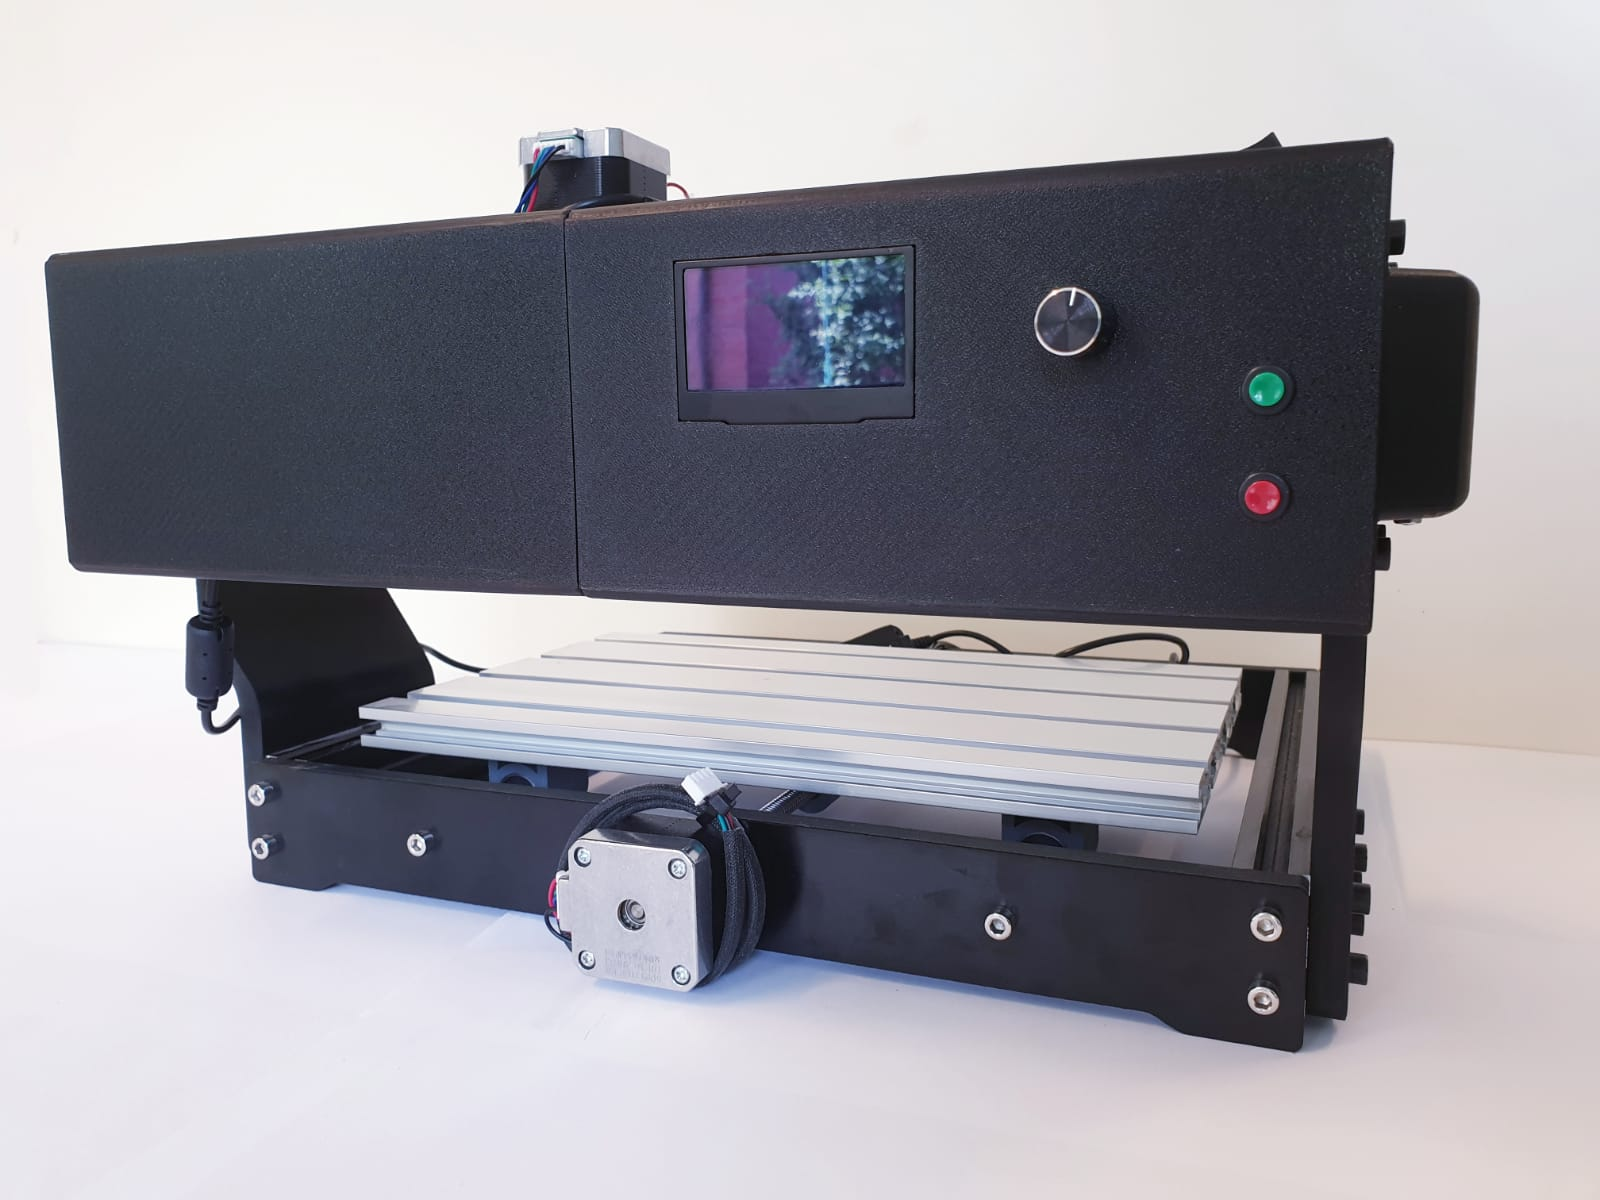
\includegraphics[width=0.9\textwidth]{Images/Montiert.jpg}
		\caption{Demonstrator Schrittmotor} \label{Montiert}
	\end{center}
\end{figure}


\section{Schalter}
\begin{figure}[H]
	\vspace{1.5cm}
	\centering
	\tikzset{short/.style={}}
	\begin{tikzpicture}[scale=0.6, 
		every node/.style={font=\fontsize{800pt}{1000pt}\selectfont\bfseries}]
			\tikzstyle{every node}=[font=\LARGE]
			\draw [line width=1pt, short] (5.25,12) -- (5.25,9.75);
			\draw [line width=1pt, short] (5.25,9.75) -- (6.25,9.25);
			\draw [line width=1pt, short] (6,10) -- (5.75,10);
			\draw [line width=1pt, short] (5.75,10) -- (5.75,11.75);
			\draw [line width=1pt, short] (6,10) -- (6,11.75);
			\draw [line width=1pt, short] (6,11.25) -- (7.25,11);
			\draw [line width=1pt, short] (7.25,11) -- (7.75,11.25);
			\draw [line width=1pt, short] (7.75,12) -- (7.75,11.25);
			\draw [line width=1pt, short] (6.25,9.25) -- (6.25,6.75);
			\draw [line width=1pt, short] (9,11) -- (9,12.75);
			\draw [line width=1pt, short] (6.25,6.75) -- (3.75,8.5);
			\draw [line width=1pt, short] (3.75,8.5) -- (2,7.5);
			\draw [line width=1pt, short] (7.75,11.25) -- (6,11.5);
			\draw [line width=1pt, short] (6.5,11.75) -- (6.5,12.25);
			\draw [line width=1pt, short] (5.25,12) -- (6.5,11.75);
			\draw [line width=1pt, short] (6.5,11.75) -- (7.75,12);
			\draw [line width=1pt, short] (6.5,12.25) -- (9,12.75);
			\draw [line width=1pt, short] (6.5,12.25) -- (3.75,12.75);
			\draw [line width=1pt, short] (3.75,12.75) -- (0.25,12);
			\draw [line width=1pt, short] (9,12.75) -- (3.75,13.5);
			\draw [line width=1pt, short] (5.75,10) -- (5.25,10.25);
			\draw [line width=1pt, short] (3.75,12.75) -- (3.75,8.5);
			\draw [line width=1pt, short] (7,8.75) -- (9,7.5);
			\draw [line width=1pt, short] (9,7.5) -- (9,10.5);
			\draw [line width=1pt, short] (7,10.75) -- (7,8.75);
			\draw [line width=1pt, short] (7,10.75) -- (7.75,11);
			\draw [line width=1pt, short] (7.75,11) -- (9.5,10.75);
			\draw [line width=1pt, short] (9,10.5) -- (9.75,10.75);
			\draw [line width=1pt, short] (9.75,10.75) -- (9.75,8.25);
			\draw [line width=1pt, short] (9,7.5) -- (9.75,8.25);
			\draw [line width=1pt, short] (6.25,9.25) -- (7,9.5);
			\draw [line width=1pt, short] (7.25,11) -- (7.25,10.75);
			\draw [line width=1pt, short] (6,10) -- (7,9.5);
			\draw [line width=1pt, short] (6.25,6.75) -- (8.25,8);
			\draw [line width=1pt, short] (7,10.75) -- (9,10.5);
			\draw [line width=1pt, short] (7,10.25) -- (6.75,10.25);
			\draw [line width=1pt, short] (6.75,10.25) -- (6.75,10);
			\draw [line width=1pt, short] (6.75,10) -- (7,10);
			\draw [line width=1pt, short] (6.75,9.75) -- (6.75,9.5);
			\draw [line width=1pt, short] (6.75,9.75) -- (7,9.75);
			\draw [line width=1pt, short] (6.75,9.5) -- (7,9.5);
			\draw [line width=1pt, short] (7,9.25) -- (6.75,9.25);
			\draw [line width=1pt, short] (6.75,9.25) -- (6.75,9);
			\draw [line width=1pt, short] (6.75,9) -- (7,9);
			\draw [line width=1pt, short] (9.5,10.75) .. controls (10.5,9.75) and (10.75,9.5) .. (9.75,8.25);
			\draw [line width=1pt, short] (9.25,10.5) .. controls (10.5,9.75) and (10,9.25) .. (9.5,8.25);
			\draw [line width=1pt, dashed] (6.75,9.5) -- (5.25,10.5);
			\draw [line width=1pt, dashed] (6.75,10.25) -- (5.25,10.75);
			\draw [line width=1pt, ->, >=Stealth, dashed] (8.5,9.25) -- (7.5,9.75);
			\draw [ line width=1pt ] (9.5,8.25) circle (0.5cm);
	\end{tikzpicture}

\caption{Endschalterposition}
\label{tikz:Endschalter}
\end{figure}

\subsection{Endschalter:}
Die Endschalter sind in den jeweiligen Gehäusekörpern zu montieren (rechter Endschalter in rechten Gehäusekörper, linker Endschalter in linken Gehäusekörper). Die Montage erfolgt von vorn, indem die Endschalter in die vorgesehenen Aufnahmen eingeschoben werden. Das Gehäuse ist so ausgelegt, dass die Schalter selbst klemmend geführt sind und an einem definierten Anschlag fixieren.

Zur Funktionsprüfung ist der Betätigungsmechanismus des Schalters leicht zu drücken. Ist ein deutliches Klickgeräusch wahrnehmbar, befindet sich der Schalter in korrekter Einbaulage. Bleibt das Geräusch aus, liegt der Schalter möglicherweise zu tief im Gehäuse, wodurch der Betätigungsbügel nicht ausreichend ausgelenkt wird. In diesem Fall ist der Schalter leicht zurückzuziehen, bis die Betätigung korrekt erfolgt.

Die Anschlussleitungen sind anschließend durch den oberen Bereich der seitlichen Gehäusearme zu führen.


\subsection{Drucktaster grün und rot:}
Zur Montage der Drucktaster im rechten Gehäusekörper ist zunächst das Spanngehäuse beider Taster zu demontieren. Anschließend werden die Anschlussleitungen des grünen Tasters von vorn durch den oberen, 9 mm großen Lochausschnitt geführt, bis das Kunststoffgehäuse des Tasters plan auf der Gehäuseoberfläche aufliegt. Danach wird das Spanngehäuse von hinten über die Kabel geschoben und wieder am Taster verschraubt.

Führen Sie diesen Vorgang für den roten Drucktaster durch. Für ihn ist der darunterliegende Lochausschnitt vorgesehen.

\subsection{Encoder}
Zur Befestigung des Encoders kann die sich an der Drehachse befindende Mutter mit Unterlegscheibe abgedreht werden, die Drehachse von Innen durch die zugehörige Öffnung geschoben und von der Frontseite, wieder mit der Unterlegscheib und MUtter fest an das Gehäusegepannt werden. Abschließend kann die Abdeckkappe aufgesteckt werden. 

\subsection{Wippschalter}
Der Wippschalter wird von außen in den vorgesehenen Ausschnitt des rechten Gehäusekörpers eingesetzt und hält sich durch Selbstklemmung in Position. 

\section{Display}
Das Display wird von innen unter die vorgesehenen Halterungen eingeschoben und richtet sich durch seine Form selbst im Gehäuseausschnitt aus.

\section{Geschwindigkeitssensor Teil 1}
Die Positionierung des Geschwindigkeitssensors erfolgt in zwei Schritten: Zunächst wird der Sensor im Gehäusekörper eingesetzt. Anschließend wird das Gehäuse angebracht, sodass der Sensor im finalen Schritt korrekt ausgerichtet werden kann.

Setzen Sie den Geschwindigkeitssensor in den Arm des rechten Gehäusekörpers ein. Die Verlegung der Kabel erfolgt analog zur des im selben Gehäuse befindlichen Endschalters.
Positionieren Sie den Sensor im verjüngten Abschnitt des Gehäusearms, um ausreichend Freiraum für die spätere Montage der Lochscheibe zu gewährleisten. Führen Sie eine Senkkopfschraube M3 durch die Bohrung der Sensorhalterung sowie die Nut im Gehäusearm. Fixieren Sie den Sensor anschließend von außen mit einer M3-Unterlegscheibe und einer M3-Mutter.

\chapter{Verkabelung aller Komponenten}

Verbinden Sie den Pol 2 der Leitungen mit der Anschlusskomponente 2 Pol 2 gemäß der in Tabelle \ref{Leittab2} dargestellten Zuordnung. Zu beachten ist die Pos.12, das Anschlusskabel wird hier von außen durch die Bohrung des linken Gehäusekörpers, nach Innen, gezogen und am Entwicklerboard angeschlossen. 
Nach dem Anschluss der Leitungen wird empfohlen, ähnliche Leitungen mithilfe von Kabelbindern zu bündeln, um eine übersichtliche Kabelführung zu gewährleisten. Zur Kürzung der überstehenden Enden der Kabelbinder verwenden Sie bitte einen geeigneten Seitenschneider.

\begin{figure}[H]
	\begin{center}
		\fontsize{8}{10}\selectfont
		\begin{tabularx}{\textwidth}{|p{0.5cm}|p{1cm}|p{2.5cm}|p{2cm}|p{2cm}|p{2cm}|p{2cm}|} 
			\hline 
			\textbf{\newline Pos.} &  \textbf{\newline Anz. pro Leitung} &  \textbf{\newline Leitungsart \newline Pol1 - Pol2} &  \textbf{\newline Anschluss- \newline komponente 1} &  \textbf{\newline Komponente 1 Pol1} & \textbf{\newline Anschluss- \newline komponente 2} &  \textbf{\newline Komponente 2 Pol2} \\ \hline
			1 & \newline 1  & \newline abisoliert - male \newline abisoliert - male & Steckerverbinder  & \newline + \newline - & Entwicklerboard & \newline 9V \newline GND \\ \hline
			2 & \newline 2  & \newline male - female \newline male - female \newline male - male & Schrittsensor & \newline VCC \newline GND \newline Out & \newline Steckbrett \newline Stekbrett \newline Arduino & \newline + \newline - \newline P9 \\ \hline
			3 & 1 & \newline abisoliert - male \newline abisoliert - male  & Taster grün & \newline + \newline - & \newline Arduino \newline Steckbrett & \newline P4 \newline -  \\ \hline
			4 & 1 & \newline abisoliert - male \newline abisoliert - male  & Taster rot & \newline + \newline - & \newline Arduino \newline Steckbrett & \newline P5 \newline -  \\ \hline
			5 & 1 & \newline abisoliert - female \newline abisoliert - male  & Powerschalter & \newline + \newline - & \newline Arduino \newline Steckbrett & \newline P8 \newline - \\ \hline
			6 & \newline 3  & \newline female - male \newline female - male \newline female - male \newline female - male \newline female - male & Encoder & \newline CLK \newline DT \newline SW \newline + \newline GND  &\newline Arduino \newline Arduino \newline Arduino \newline Steckbrett \newline Steckbrett &\newline A1 \newline A2 \newline A3 \newline + \newline - \\ \hline
			7 & \newline 3  & \newline abisoliert - male \newline abisoliert - male & Endschalter rechts & \newline NC \newline C &  \newline Arduino \newline Steckbrett & \newline P7 \newline -  \\ \hline
			8 & \newline 3  & \newline abisoliert - male \newline abisoliert - male & Endschalter links & \newline NC \newline C &  \newline Arduino \newline Steckbrett & \newline P11 \newline -  \\ \hline
			9 & \newline 1   & \newline female - male \newline female - male \newline female - male \newline female - male \newline female - male \newline female - male \newline female - male  & Display & \newline D2 \newline A0 \newline RST \newline D1 \newline D0 \newline VDD \newline VSS & \newline Arduino \newline Arduino \newline Arduino \newline Arduino \newline Arduino \newline Steckbrett \newline Steckbrett & \newline P6 \newline P12 \newline P10 \newline A4 \newline A5 \newline + \newline - \\ \hline
			10 & \newline 1  & \newline female - male \newline female - male  & Arduino & \newline 5V \newline GND & \newline Steckbrett \newline Steckbrett & \newline + \newline -  \\ \hline
			11 & \newline 1 & \newline male - male \newline male - male \newline male - female \newline male - female  & Entwicklerboard & \newline 5V \newline GND \newline 9 \newline 8  & \newline Steckbrett \newline Steckbrett \newline Arduino \newline Arduino & \newline + \newline - \newline P3 \newline P2 \\ \hline
			12 & \newline bestehen- \newline des Anschlusskabel & \newline x - female & Schrittmotor & A1,A2,B1,B2 & Entwicklerboard & \newline Anschluss- \newline buchse  \\ \hline
			
			
		\end{tabularx}
		\captionof{table}{Leitungen}	\label{Leittab2}
	\end{center}
\end{figure}


\section{Schaltplan}
Die Verkabelung sollte nun dem Schaltplan aus Abb.\ref{Leitungen} entsprechen.

\begin{figure}[H]
	\begin{center}
		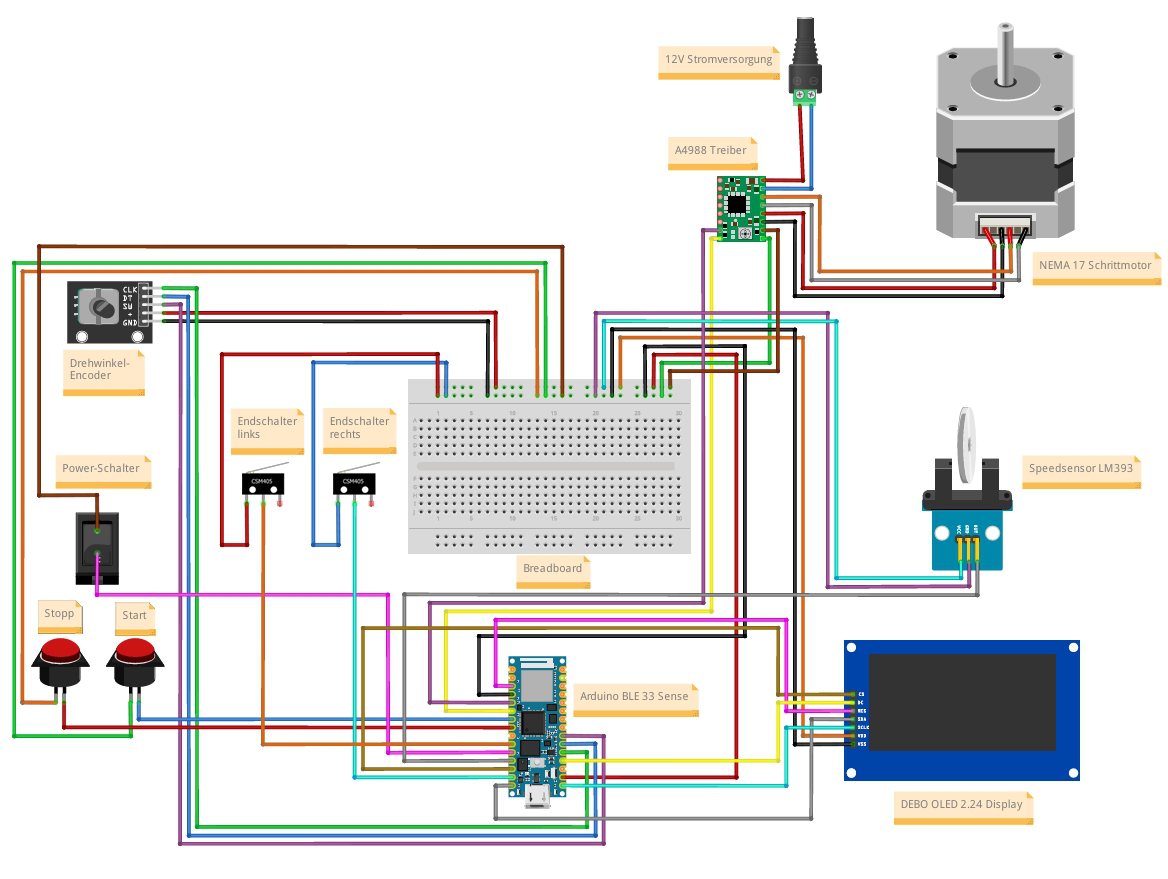
\includegraphics[width=\textwidth]{Images/Schaltplan.jpeg}
		\caption{Schaltplan} \label{Leitungen}
	\end{center}
\end{figure}


\chapter{Einhängung der Gehäusehälften}
Die Einhängung der Gehäusekörper wird im Folgenden anhand der linken Hälfte erklärt und kann für die rechte Hälfte übernommen werden. 
Richten Sie das Gehäuse versetzt zu Seitenträger und Profile erhöht aus, Abb \ref{fig:positionierung_gehaeuse1}.

\begin{figure}[H]
	\centering
	\begin{minipage}{0.48\linewidth}
		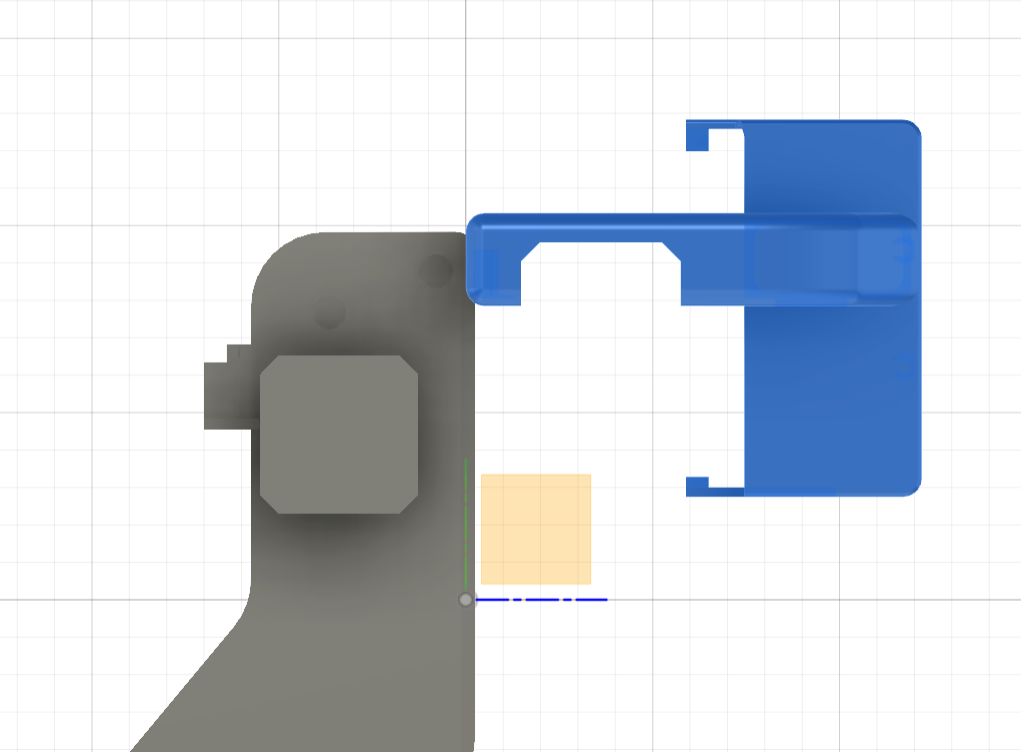
\includegraphics[width=\linewidth]{Images/Positionierung1.2.png}
		\caption*{Bild 1: Ausrichtung Z}
	\end{minipage}
	\hfill
	\begin{minipage}{0.48\linewidth}
		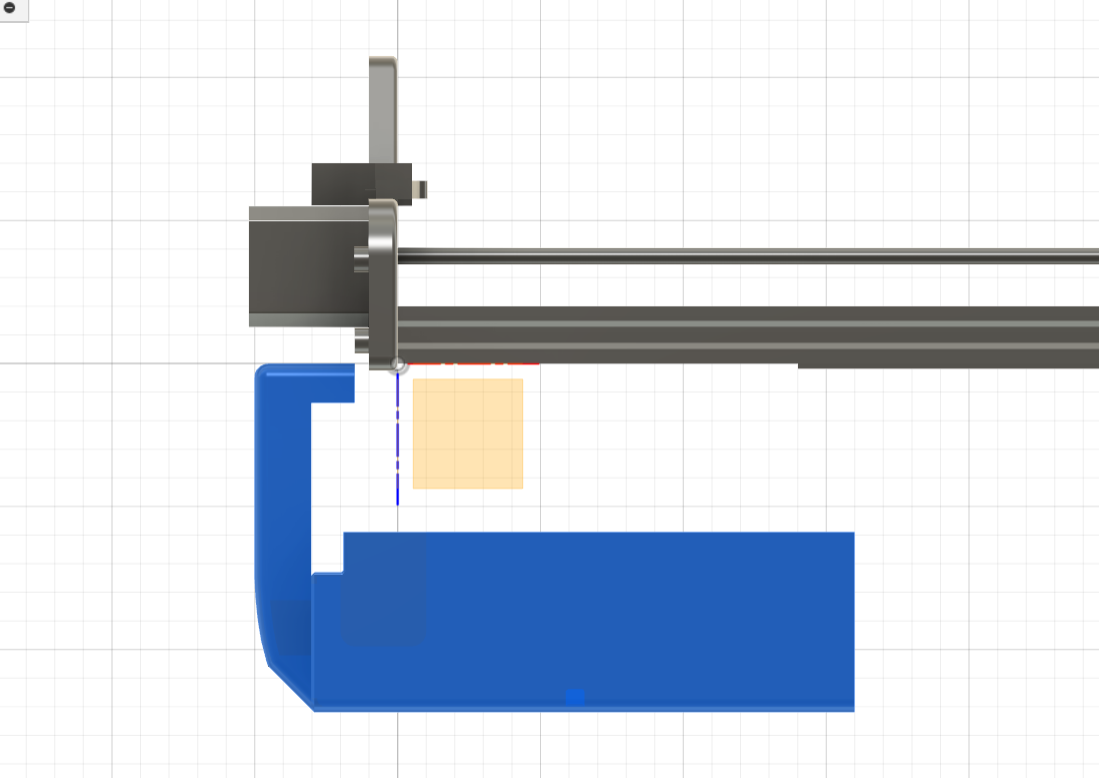
\includegraphics[width=\linewidth]{Images/Positionierung1.png}
		\caption*{Bild 2:Ausrichtung Y}
	\end{minipage}
	\caption{Positionierungen zur Einhängung 1}
	\label{fig:positionierung_gehaeuse1}
\end{figure}

Nähern Sie sich dem CNC-Tisch. Das Gehäuse muss vorsichtig nach außen gebogen werden, damit die Halter über die Seitenteile der Profile hinweg in die entsprechende Nut eingesetzt werden können, Abb \ref{fig:positionierung_gehaeuse2}.
	\vspace{0.5cm}
\begin{figure}[H]
	\centering
	\begin{minipage}{0.48\linewidth}
		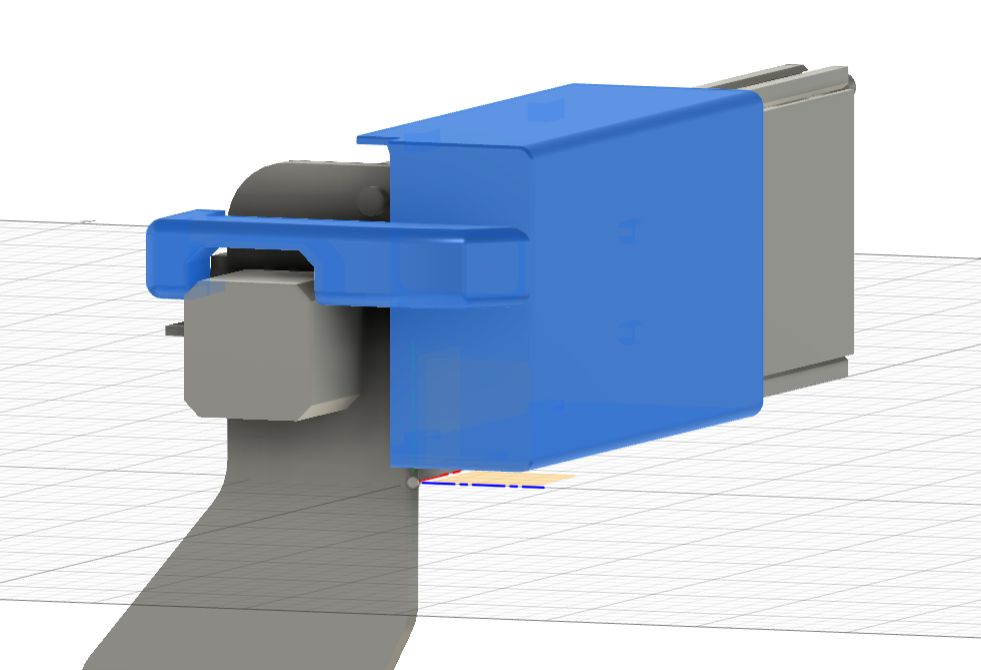
\includegraphics[width=\linewidth]{Images/Positionierung2.png}
		\caption*{Bild 1: Näherung}
	\end{minipage}
	\hfill
	\begin{minipage}{0.48\linewidth}
		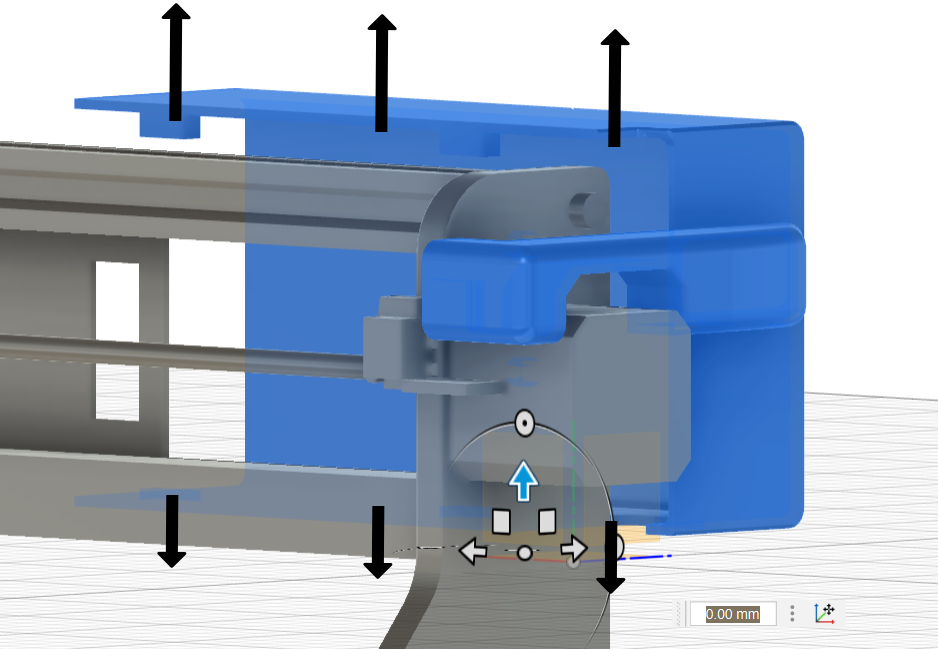
\includegraphics[width=\linewidth]{Images/Positionierung3.png}
		\caption*{Bild 2: Biegung des Gehäuses }
	\end{minipage}
	\caption{Positionierungen zur Einhängung 2}
	\label{fig:positionierung_gehaeuse2}
\end{figure}
	\vspace{0.5cm}
Nachdem das Gehäuse korrekt in die Nut eingehakt wurde, kann es in Richtung der Spindel über den Schrittmotor hinweg an den Seitenträger geschoben werden. Achten Sie dabei auf die Zylinderkopfschrauben des Seitenträgers, welche den Gehäusearm zusätzlich in Position halten
	\vspace{0.5cm}.
\begin{figure}[H]
	\centering
	\begin{minipage}{0.32\linewidth}
		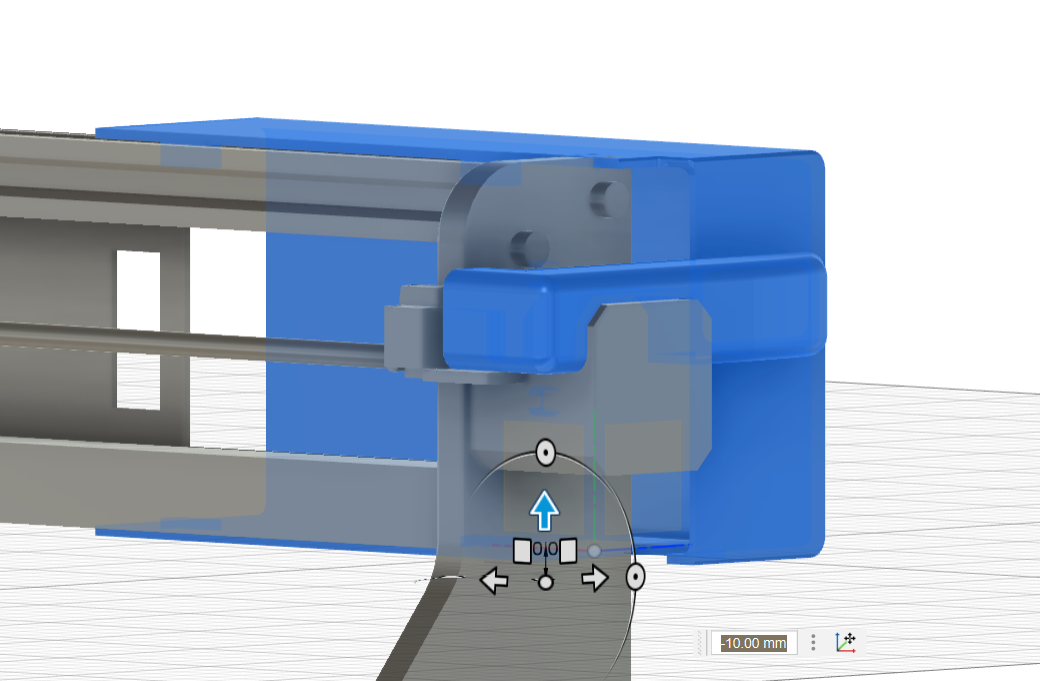
\includegraphics[width=\linewidth]{Images/Positionierung4.png}
		\caption*{Bild 1: Aufsatz}
	\end{minipage}
	\hfill
	\begin{minipage}{0.32\linewidth}
		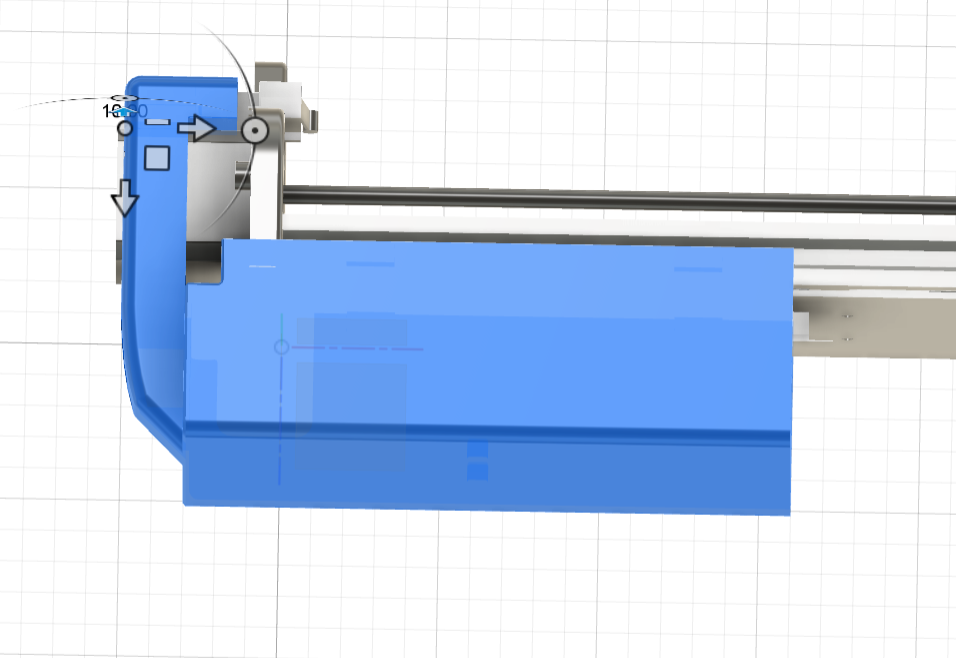
\includegraphics[width=\linewidth]{Images/Positionierung5.png}
		\caption*{Bild 2: Einschieben}
	\end{minipage}
		\hfill
	\begin{minipage}{0.32\linewidth}
		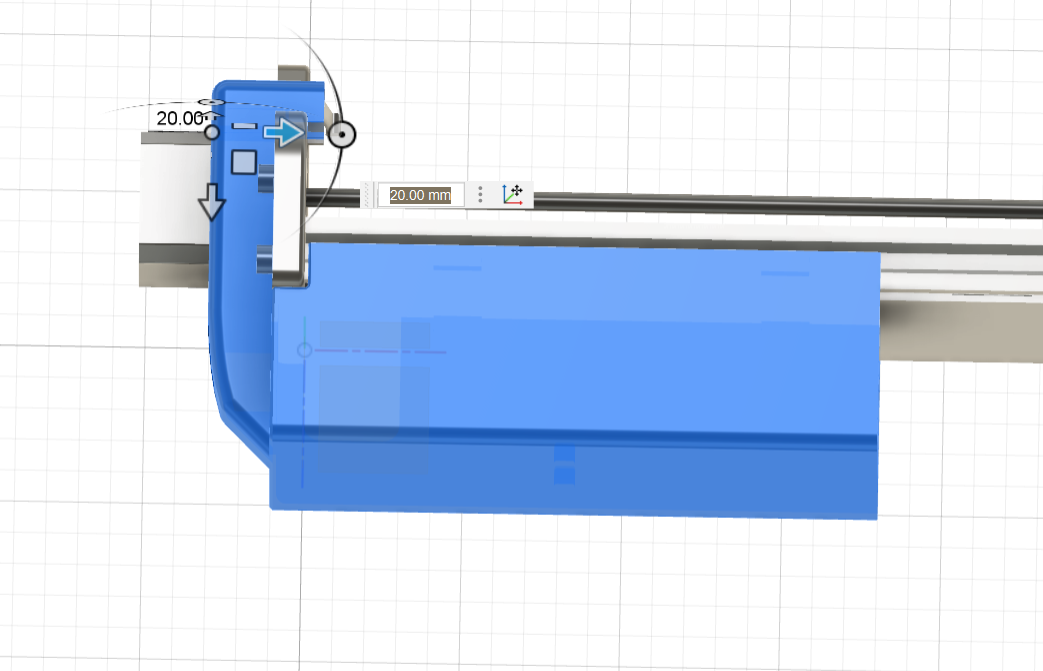
\includegraphics[width=\linewidth]{Images/Positionierung5.2.png}
		\caption*{Bild 2: Einschieben}
	\end{minipage}
	\caption{Positionierungen zur Einhängung 3}
	\label{fig:positionierung_gehaeuse3}
\end{figure}
	\vspace{0.5cm}
Wiederholen Sie den Prozess für die rechte Seite und achten Sie darauf, dass sich keine Kabel lösen.


\chapter {Ausrichtung des Geschwindigkeitssensor}



\section{Geschwindigkeitssensor Teil 2}
Lösen Sie die Mutter des Geschwindigkeitssensors und verschieben Sie den Sensor entlang der Nut um 20 mm nach hinten, sofern Sie das Originalgehäuse verwenden. Stoppen Sie die Verschiebung auf Höhe der Markierung und ziehen Sie die Mutter anschließend wieder fest.\\

Der Sensor ist nun korrekt positioniert, sodass sich die Lochscheibe zwischen den Messarmen des Sensors befindet.




\chapter{Prüfung}

	\item Testen Sie Mithilfe des Handbuchs die Funktionsfähigkeit des Demonstrators. 

